\documentclass{article}
\usepackage{amsmath}
\usepackage{circuitikz}

\title{AP Physics C: Chapter 22}
\author{Zach Baylin}

\begin{document}
\maketitle
\section{Charge Model}
\begin{itemize}
  \item Two types of charge exist
    \begin{itemize}
      \item $(+)$: proton $N_p$
      \item $(-)$: proton $N_e$
    \end{itemize}
  \item Unit is \textbf{Coulombs} ($Q, q$)
  \item $e$ is the \textbf{fundamental charge}: $1.6\times10^{-19}$
  \item \textbf{neutral object}: some number of $N_p$ and $N_e$
  \item \textbf{charged object}: an imbalance of electrons: $q=N_p e - N_e e$
  \item \textit{N.B. charge is quantized: increases or decreases in discrete jumps}
  \item Electrons transfer to other object but charge is conserved
  \item Opposites attract
  \item Two types of electromagnetic matter
    \begin{itemize}
      \item \textbf{conductors}: electrons are free to move
        \begin{itemize}
          \item \begin{tabular}{ccccc}
                  & $(-)$ & $(-)$ & $(-)$ &     \\
            $(-)$ & $(+)$ & $(+)$ & $(+)$ & $(-)$ \\
            $(-)$ & $(+)$ & $(+)$ & $(+)$ & $(-)$ \\
            $(-)$ & $(+)$ & $(+)$ & $(+)$ & $(-)$ \\
                  & $(-)$ & $(-)$ & $(-)$ &    
          \end{tabular}
          \item \textbf{sea of electrons}
          \item Valence electrons
          \item Mostly metals
          \item They charge by \textbf{conduction} (touching)
            \begin{itemize}
              \item Results in a shift of the sea of electrons
              \item Charge is excessive and equally distributed
              \item An object with the same charge as the other
              \item \textbf{electrostatic equilibrium}: charge is equally distributed, on the surface, and at rest
            \end{itemize}
        \end{itemize}
      \item \textbf{insulators}: electrons are \underline{not} free to move
        \begin{itemize}
          \item \begin{tabular}{cccccc}
            $(+)$ & $(-)$ & $(+)$ & $(-)$ & $(+)$ & $(-)$
            \end{tabular}
          \item valence $e^-$ tightly bonded to proton
          \item When they are rubbed together, the degree of their opposite charge depends on their measurement on the \textbf{triboelectric scale}
        \end{itemize}
    \end{itemize}
    \item \textbf{electrostatic discharge} requires contact with a conductor
      \begin{itemize}
        \item if conductor to conductor (\textbf{grounding}) \begin{circuitikz}
          \draw node[ground]{}; 
        \end{circuitikz}
      \end{itemize}
    \item \textbf{polarization}: neutral object with same number of $N_p$ and $N_e$, but one side is ``more positive'' and the other ``more negative''
    \item \textbf{charging by induction}: only occurs in conductors
      \begin{itemize}
        \item Occurs when a charged object is brought near a grounded conductor.
        \item Electrons are lost along the grounded wire.
        \item Removing ground wire results in a conductor with positive charge in electrostatic equilibrium.
      \end{itemize}
\end{itemize}
\section{Point Charge}
\begin{itemize}
  \item Conceptually shrinking down an object so that it has mass and charge but no size
  \item We can quantify how much force two charges experience with $\dfrac{k\cdot|q_1||q_2|}{r^2}$
    \begin{itemize}
      \item $k=K=K_E$
      \item $k=8.99\times 10 ^{9}$
    \end{itemize}
  \item \begin{tikzpicture}
    \draw[->] node{$+q_1$} (.4,0) -- (1,0); 
    \draw[->] (2.6,0) -- (2,0);
    \draw (3,0) node{$-q_2$};
  \end{tikzpicture}
  \item 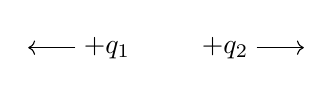
\begin{tikzpicture}
    \draw[->] (.7,0) -- (.1,0);
    \draw (1.1,0) node{$+q_1$};
    \draw[->] (3,0) -- (3.6,0);
    \draw (2.6,0) node{$+q_2$};
  \end{tikzpicture}
\end{itemize}
\section{Electric Field}
\begin{itemize}
  \item Charge causes a change in the space around it, which becomes a vector field
  \item $\vec{E}=\dfrac{1}{4\pi t_0}\cdot\dfrac{Q}{r^2}\cdot\vec{r}$
  \item $F_{E_q}=\dfrac{1}{r\pi t_0}\cdot\dfrac{qQ}{r^2}\cdot\vec{r}=q\vec{E}$
\end{itemize}
\end{document}